\documentclass{article}
\usepackage{hyperref}

\usepackage{graphicx}
\usepackage{amssymb}
\usepackage{epstopdf}
\DeclareGraphicsRule{.tif}{png}{.png}{`convert #1 `dirname #1`/`basename #1 .tif`.png}

\title{Charlie Tanksley}
\date{\today}


\begin{document}
\maketitle

\section{Web Presence} % {{{
\label{sec:Web Presence}

\begin{itemize}
  \item Github 
    \href{https://github.com/charlietanksley}{https://github.com/charlietanksley}
  \item Homepage 
    \href{http://www.charlietanksley.net}{http://www.charlietanksley.net}
  \item General Programming Blog
    \href{http://www.charlietanksley.net/blog}{http://www.charlietanksley.net/blog}
  \item \LaTeX\ Blog (group blog)
    \href{http://www.charlietanksley.net/philtex}{http://www.charlietanksley.net/philtex}
\end{itemize}

% section Web Presence }}}
\section{Contact} % {{{
\label{sec:Contact}

\begin{itemize}
  \item 
    \href{mailto:charlie.tanksley@gmail.com}{charlie.tanksley@gmail.com}
  \item \href{http://www.twitter.com/charlietanksley}{@charlietanksley 
    on Twitter}
\end{itemize}

% section Contact }}}
\section{Devleopment Skills} % {{{
\label{sec:Devleopment Skills}

\subsection{Languages} % {{{
\label{sub:Languages}

\begin{itemize}
  \item Ruby
\end{itemize}

% subsection Languages }}}
\subsection{Web Frameworks} % {{{
\label{sub:Web Frameworks}

\begin{itemize}
  \item Sinatra
  \item Padrino
  \item Rails
  \item Wordpress
\end{itemize}

% subsection Web Frameworks }}}
\subsection{Markup Languages, Pre-processors, \& Tools} % {{{
\label{sub:Markup Languages, Pre-processors, \& Tools}

\begin{itemize}
  \item HTML
  \item CSS
  \item Compass
  \item Sass/Scss
  \item Haml
  \item Slim
  \item Susy (responsive grid)
  \item Goldilocks (responsive framework)
\end{itemize}

% subsection Markup Languages, Pre-processors, \& Tools }}}
\subsection{Development Tools} % {{{
\label{sub:Development Tools}

\begin{itemize}
  \item Git
  \item \LaTeX\ (typesetting system)
  \item Rspec (testing framework)
  \item Riot (testing framework)
\end{itemize}

% subsection Development Tools }}}

% section Skills }}}
\section{Recent Projects} % {{{
\label{sec:Recent Projects}

\subsection{Moxie Academy} % {{{
\label{sub:Moxie Academy}

\href{http://www.moxieacademy.com}{http://www.moxieacademy.com}

\begin{description}
  \item[description] Moxie Academy is the front-end for an online 
    course.  The course content includes bith text and videos, so the 
    outward facing site must display both (and the admin interface 
    must allow the adminstrator to interact with both).
  \item[responsibilities] all coding (front-end and back-end), design, and graphics
  \item[technologies] Ruby, Padrino, Compass, Sass, Susy (responsive framework), DataMapper, Slim, Heroku
\end{description}


\includegraphics[scale=.5]{../source/images/portfolio/moxie-homepage-sm.png}
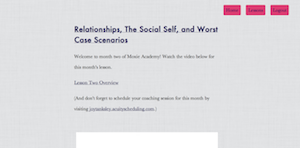
\includegraphics[scale=.5]{../source/images/portfolio/moxie-lesson-sm.png}
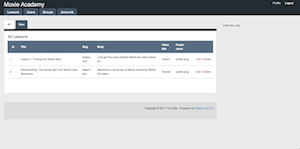
\includegraphics[scale=.5]{../source/images/portfolio/moxie-admin-sm.png}

% subsection Moxie Academy }}}
\subsection{ThePhilosopher.me} % {{{
\label{sub:ThePhilosopher.me}

\href{http://www.thephilosopher.me}{http://www.thephilosopher.me}

\begin{description}
  \item[description] ThePhilosopher.me was designed with one goal: to 
    enable non-technical people (philosophers!) to create simple, 
    informative, topical personal sites.  Since the most important 
    facts about philosophers are their contact information and 
    publications, this application aims to make it as easy as possible 
    to create a page with both.  The publication data comes from an 
    external source via screen scraping (to obviate the need for 
    time-consuming data entry).
  \item[responsibilities] idea, all coding (front-end and back-end), 
    design, and graphics
  \item[technologies] Ruby, Sinatra, MongoDB, Mongoid, Compass, Sass, 
    Susy, Haml, Heroku, MongoHQ
\end{description}

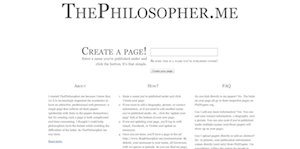
\includegraphics[scale=.5]{../source/images/portfolio/philosopher.me-home-sm.png}

\includegraphics[scale=.5]{../source/images/portfolio/philosopher.me-sample-sm.png}

% subsection ThePhilosopher.me }}}
\subsection{Fierce Love} % {{{
\label{sub:Fierce Love}

\href{http://www.fiercelove.me}{http://www.fiercelove.me}

\begin{description}
  \item[description] Fierce Love is an umbrella site for a series of courses offered by a life-coaching team.  At present, the site is written on top of WordPress.  The current course has lessons that are text, video, and/or audio.  The site uses custom roles to display content to users at the appropriate time in their course.
  \item[responsibilities] all coding (front-end and back-end), design, and graphics (save main logo)
  \item[technologies] PHP, WordPress, Compass, Sass
\end{description}

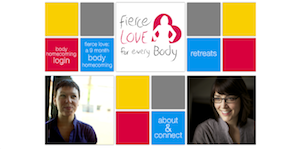
\includegraphics[scale=.5]{../source/images/portfolio/fierce-love-homepage-sm.png}
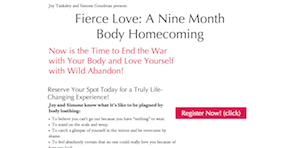
\includegraphics[scale=.5]{../source/images/portfolio/fierce-love-sales-sm.png}

% subsection Fierce Love }}}
\subsection{Joy Tanksley's Coaching Site} % {{{
\label{sub:Joy Tanksley's Coaching Site}


\href{http://www.joytanksley.com}{http://www.joytanksley.com}

\begin{description}
  \item[description] A business site and blog for a life coach. 
  \item[responsibilities] all coding (front-end and back-end), design, and graphics 
  \item[technologies] StaticMatic (Ruby static site generator), WordPress, Haml, Compass, Sass, jQuery 
\end{description}


\includegraphics[scale=.5]{../source/images/portfolio/joytanksley-about-sm.png}

\includegraphics[scale=.5]{../source/images/portfolio/joytanksley-blog-sm.png}
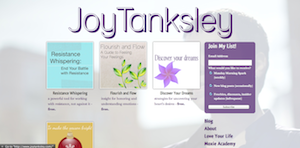
\includegraphics[scale=.5]{../source/images/portfolio/joytanksley-products-sm.png}

% subsection Joy Tanksley's Coaching Site }}}
\subsection{My Personal Site} % {{{
\label{sub:My Personal Site}

\href{http://www.charlietanksley.net}{http://www.charlietanksley.net}

\begin{description}
  \item[description] My personal site. 
  \item[responsibilities] all coding (front-end and back-end), design, and graphics 
  \item[technologies] MiddleMan (Ruby static site generator), Compass, Scss, Goldilocks Responsive Framework, Slim, Whiskey Disk (for deployment)
\end{description}

% \includegraphics[scale=.5]{../source/images/portfolio/.png}

% subsection My Personal Site }}}

% section Recent Projects }}}
\section{OSS Contributions} % {{{
\label{sec:OSS Contributions}
  \subsection{thumblemonks/riot} % {{{
  \label{sub:thumblemonks/riot}

  \begin{itemize}
    \item2011-09-13 remove mention of deprecated exists from README (1b90c5e)
    \item2011-09-13 add deprecation warning to exists macro (7201941)
    \item2011-09-03 remove mention of any macro from README (cc99cd9)
    \item2011-09-03 add deprecation warning to any macro (9b1510c)
    \item2011-09-03 remove discussion of not! from README. (3877864)
    \item2011-08-22 remove depreciated not! assertion macro (64bc72f)
  \end{itemize}

  % subsection thumblemonks/riot }}}
  \subsection{rubinius/rubinius} % {{{
  \label{sub:rubinius/rubinius}

  \begin{itemize}
    \item2011-10-15 update String#squeeze and #squeeze! specs for 19 (e804060)
    \item2011-10-15 patch String#squeeze for 19 (7acb876)
  \end{itemize}
  
  % subsection rubinius/rubinius }}}
  \subsection{davetron5000/methadone} % {{{
  \label{sub:davetron5000/methadone}
  
  \begin{itemize}
    \item2012-01-22 add features to ensure gemspec consistency (998ec00)
    \item2012-01-21 update gemspec dependencies due to bundler changes (0cc4b68)
  \end{itemize}

  % subsection davetron5000/methadone }}}

% section OSS Contributions }}}
\section{Relevant Work History} % {{{
\label{sec:Relevant Work History}

  \subsection{Sourcescape, Dec.\ 2011--Feb.\ 2012} % {{{
  \label{sub:Sourcescape}
  
  % subsection Sourscape }}}

% section Relevant Work History }}}
\section{Education} % {{{
\label{sec:Education}

\begin{itemize}
  \item 2009: Ph.D. in Philosophy, University of Virginia
  \item 2004: M.A. in Philosophy, Texas A\&M University
  \item 2002: B.A. in Philosophy, Samford University
\end{itemize}
% section Education }}}

\end{document}
